\clearpage
% \setcounter{page}{1}
\maketitlesupplementary

\section{Analytical Jacobians}

In this section, we derive analytical Jacobians used in second-order optimisation for both the tracking and backend.  For more information on Lie algebra and relevant Jacobians, please see the following \cite{sola_micro_2018, teed2021tangent}.

To take the derivatives on Lie groups with respect to the minimal parameterisation, we use the left-Jacobian definition:
\bea
\frac{\cD f(\matT)}{\cD \matT} &\triangleq \lim_{\vectau \rightarrow 0} \frac{f(\vectau \oplus \matT) \ominus f(\matT)}{\vectau}~,\\
&= \lim_{\vectau \rightarrow 0} \frac{\text{Log}\left(f\left(\text{Exp}(\vectau)\circ \matT\right) \circ f(\matT)^{-1}\right)}{\vectau}.
\eea

\subsection{Points}

For the point alignment used in both tracking and mapping, we have a residual defined between a measured point in one frame and a transformed point matched from a different frame. Using the general notation from the backend for point alignment, and switching the order of the residual which does not affect the cost function, the residual is:
\beq
r_p = \Tij \Xcanonjjn - \Xcanoniim.
\eeq
Defining $\vecx = \Tij \Xcanonjjn$ for brevity in deriving Jacobians for a single point, we take the partial derivatives with respect to the Lie algebra perturbation of the relative pose $\Tij$:
\beq
    \frac{\cD r_p}{\cD \Tij} = \begin{bmatrix} \mbf{I}_{3\times 3} & -[\vecx]_{\times} & \vecx \end{bmatrix}
    \label{eq:point_jac}
\eeq
where $[\vecx]_{\times}$ is the $3\times3$ skew-symmetric matrix.

\subsection{Rays and Distance}

Compared to the point residual, the ray residual minimises the error in normalised space, which is equivalent to minimising the angle between rays in the camera's frame:
\beq
r_\psi = \ray{\Tij \Xcanonjjn} - \ray{\Xcanoniim}.
\eeq
The Jacobian now is the chain rule of the Jacobian for normalising a point to a unit vector and Jacobian of the the pose acting on the point:
\beq
    \frac{\cD _\psi}{\cD \Tij} = \pdiff{r_\psi}{\vecx} \frac{\cD \vecx}{\cD \Tij}.
\eeq
Defining the distance from the origin of camera $i$ to point $\vecx$ as $d_{\vecx}$, the Jacobian of the first term becomes:
\beq
    \pdiff{r_\psi}{\vecx} = \frac{1}{d_{\vecx}} \left( \mbf{I}_{3\times 3} - \frac{\vecx \vecx^T}{d_{\vecx}^2} \right).
    \label{eq:norm_jac}
\eeq
Using the chain rule with \cref{eq:point_jac}, the first term becomes \cref{eq:norm_jac} itself.  Since the cross product of a point with itself is a zero vector, the second term becomes a scaled version of the skew-symmetric matrix.  Lastly, as \cref{eq:norm_jac} has the form of an operator that takes the difference between a point and its orthogonal projection onto a subspace, and projecting a point onto its own subspace preserves the point, this cancels to a zero vector.  In matrix form, this is:
\beq
    \frac{\cD r_\psi}{\cD \Tij} = \begin{bmatrix} \pdiff{r_\psi}{\vecx} & -\frac{1}{d_{\vecx}} [\vecx]_{\times} & \mbf{0}_{3 \times 1} \end{bmatrix}.
\eeq
As mentioned in the main paper, we also include an error based on the distance between the transformed point and its match so that cases with pure rotation do not result in a degenerate optimisation problem.  This error is:
\beq
    r_d = d\left(\Tij \Xcanonjjn \right) - d\left( \Xcanoniim \right)
\eeq
and its corresponding Jacobians are:
\bea
    \pdiff{r_d}{\vecx} &= \frac{\vecx^T}{d_{\vecx}}, \\
    \frac{\cD r_d}{\cD \Tij} &= \begin{bmatrix} \frac{\vecx^T}{d_{\vecx}} & \mbf{0}_{1 \times 3} & d_{\vecx} \end{bmatrix}.
    \label{eq:dist_jac}
\eea

\begin{figure*}[t]
\centering
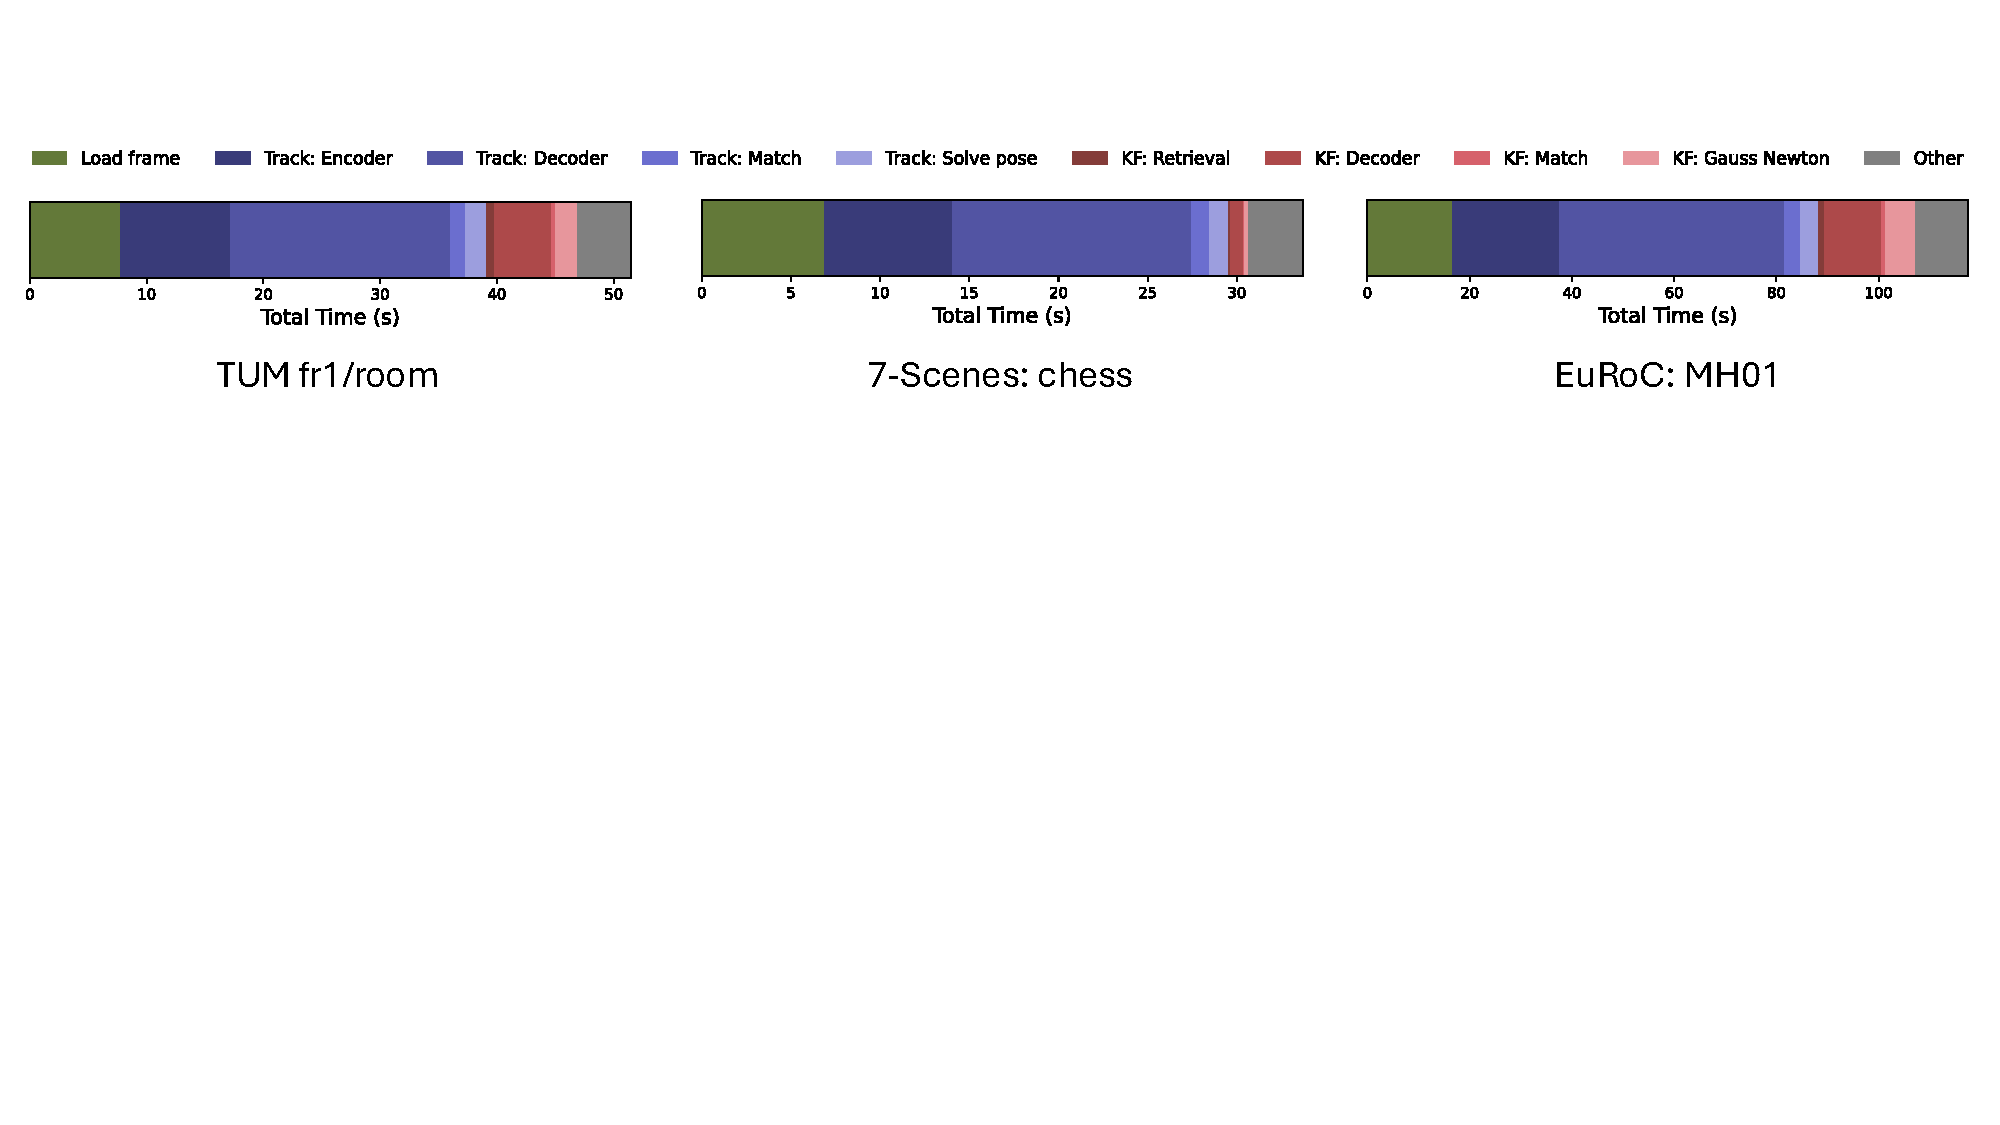
\includegraphics[width=\linewidth]{figs/timing.pdf}
\caption{Total runtime in seconds for representative datasets showing cumulative time spent in significant components.  The network encoder and decoder are the majority of the runtime at an average of 64\% of the total runtime.  Datasets with more loop closures like fr1/room and MH01 show more time spent in the backend.}
\label{fig:timing_results}
\end{figure*}

\begin{table*}[t]\centering
\caption{Average runtimes in milliseconds of different components for our single-threaded system.}\label{tab:timing}
\footnotesize
\begin{tabular}{l V{3} c V{2} cccc|c V{2} cccc|c V{3} cc}
& Data &\multicolumn{5}{c V{2}}{Per-Frame Tracking} &\multicolumn{5}{c V{3}}{Per Keyframe} & \multicolumn{2}{c}{Summary} \\
    &\multicolumn{1}{c V{2}}{Load frame} &Encoder &Decoder &Match &Solve pose &\multicolumn{1}{c V{2}}{Total} &Retrieval &Decoder &Match &Gauss-Newton &\multicolumn{1}{c V{3}}{Total} & Total time (s) & FPS \\
\hline
TUM: fr1/room &11.4 &13.8 &27.7 &1.9 &2.7 &48.6 &14.4 &\ \ 97.7 &5.8 &37.8 &157.4 &51.5 &13.2 \\
7-Scenes: chess &13.8 &14.4 &26.9 &2.0 &2.1 &47.9 &14.4 &\ \ 70.6 &4.5 &22.7 &114.0 &33.7 &14.8 \\
EuRoC: MH01 &\ \ 9.1 &11.4 &23.9 &1.7 &1.8 &41.1 &15.1 &130.4 &8.4 &66.8 &223.3 &117.6 &15.7 \\
\hline
Average &11.4 &13.2 &26.2 &1.9 &2.2 &45.9 &14.6 &\ \ 99.5 &6.2 &42.4 &164.9 &67.6 &14.6 \\
\bottomrule
\end{tabular}
\end{table*}

\subsection{Projection and Depth}

In the case of known calibration, we instead use a pixel error instead of ray error.  While the rays could also be constrained to the known camera model, we chose to use pixel error as this better models the noise distribution in pixel-level correspondence and is standard in bundle adjustment.  The pixel error is defined as:
\beq
    r_\projection = \proj{\Tij \Xcanonjjn} - \pix^i_{i,m}.
\eeq
Using a pinhole camera model with calibration
\beq
    K = \begin{bmatrix} f_x & 0 & c_x \\ 0 & f_y & c_y \\ 0 & 0 & 1 \end{bmatrix},
\eeq
the projection Jacobian of point $\vecx = [x,y,z]^T$ is
\beq
    \pdiff{r_\projection}{\vecx} = \frac{1}{z} \begin{bmatrix} f_x & 0 & -f_x \frac{x}{z} \\ 0 & f_y & -f_y \frac{y}{z} \end{bmatrix}.
\eeq
We can then obtain $\frac{\cD r_\projection}{\cD \Tij}$ via the chain rule with \cref{eq:point_jac}.  We also include a small error on the predicted and measured depth with similar motivation to \cref{eq:dist_jac} in cases of pure rotation.  In the future, any parametric camera model and its corresponding Jacobian could be used here.

\subsection{From Relative Pose to Global Pose}

While the above derivations show the Jacobians with respect to relative camera poses, we ultimately need updates with respect to camera poses in the world frame.
Using $\Tij=\Twci^{-1}\Twcj$ and the identities for the left Jacobian of the group inverse and composition
\bea
    \frac{\cD \Twci^{-1}}{\cD \Twci} &= -\text{Ad}_{\Twci^{-1}}, \\
    \frac{\cD \Tij}{\cD \Twci^{-1}} &= \mbf{I}_{7\times 7}, \\
    \frac{\cD \Tij}{\cD \Twcj} &= \text{Ad}_{\Twci^{-1}},
\eea
we can then solve for updates to each pose:
\bea
    \frac{\cD r_\psi}{\cD \Twci} &= \frac{\cD r_\psi}{\cD \Tij} \frac{\cD \Tij}{\cD \Twci} = - \frac{\cD r_\psi}{\cD \Tij} \text{Ad}_{\Twci^{-1}}, \\
    \frac{\cD r_\psi}{\cD \Twcj} &= \frac{\cD r_\psi}{\cD \Tij} \frac{\cD \Tij}{\cD \Twcj} = \frac{\cD r_\psi}{\cD \Tij} \text{Ad}_{\Twci^{-1}}.
\eea

\section{Initialisation}
As mentioned in \cref{sec:tracking}, to minimise the number of network passes required for tracking, we re-use the last keyframe's pointmap estimate $\Xcanonkk$.
Such pointmap is always available, apart from at the initialisation.
To initialise the system, we simply feed the same image into \master to perform monocular prediction of the pointmap.
While such monocular predictions are often inaccurate, the pointmap incorporates multiview information and is refined using the running weighted average filter.

\section{Runtime Breakdown}

We report the cumulative runtime for different components of our system across three representative datasets in \cref{fig:timing_results}.  We also show average runtimes of different components in \cref{tab:timing}.  Note that tracking, which operates at greater than 20 FPS, occurs for every frame while keyframing is dependent on the motion and thus occurs at a lower frequency.  In general, the network encoder and decoder are the most significant in terms of time spent for both the tracking and backend at around 64\% of the total runtime.  As a large number of loop closures are detected in TUM fr1/room and EuRoC MH01, the time spent in the backend increases compared to the more linear trajectory in 7-Scenes chess.  Our efficient matching, tracking, and backend optimisation ensure that we can achieve real-time performance, with the network currently being the limiting factor on lower-latency SLAM.  The combination of the modular prior and principled backend optimisation achieves global consistency in real-time.

\section{Evaluation Setup}

\begin{figure*}[t]
    \centering
    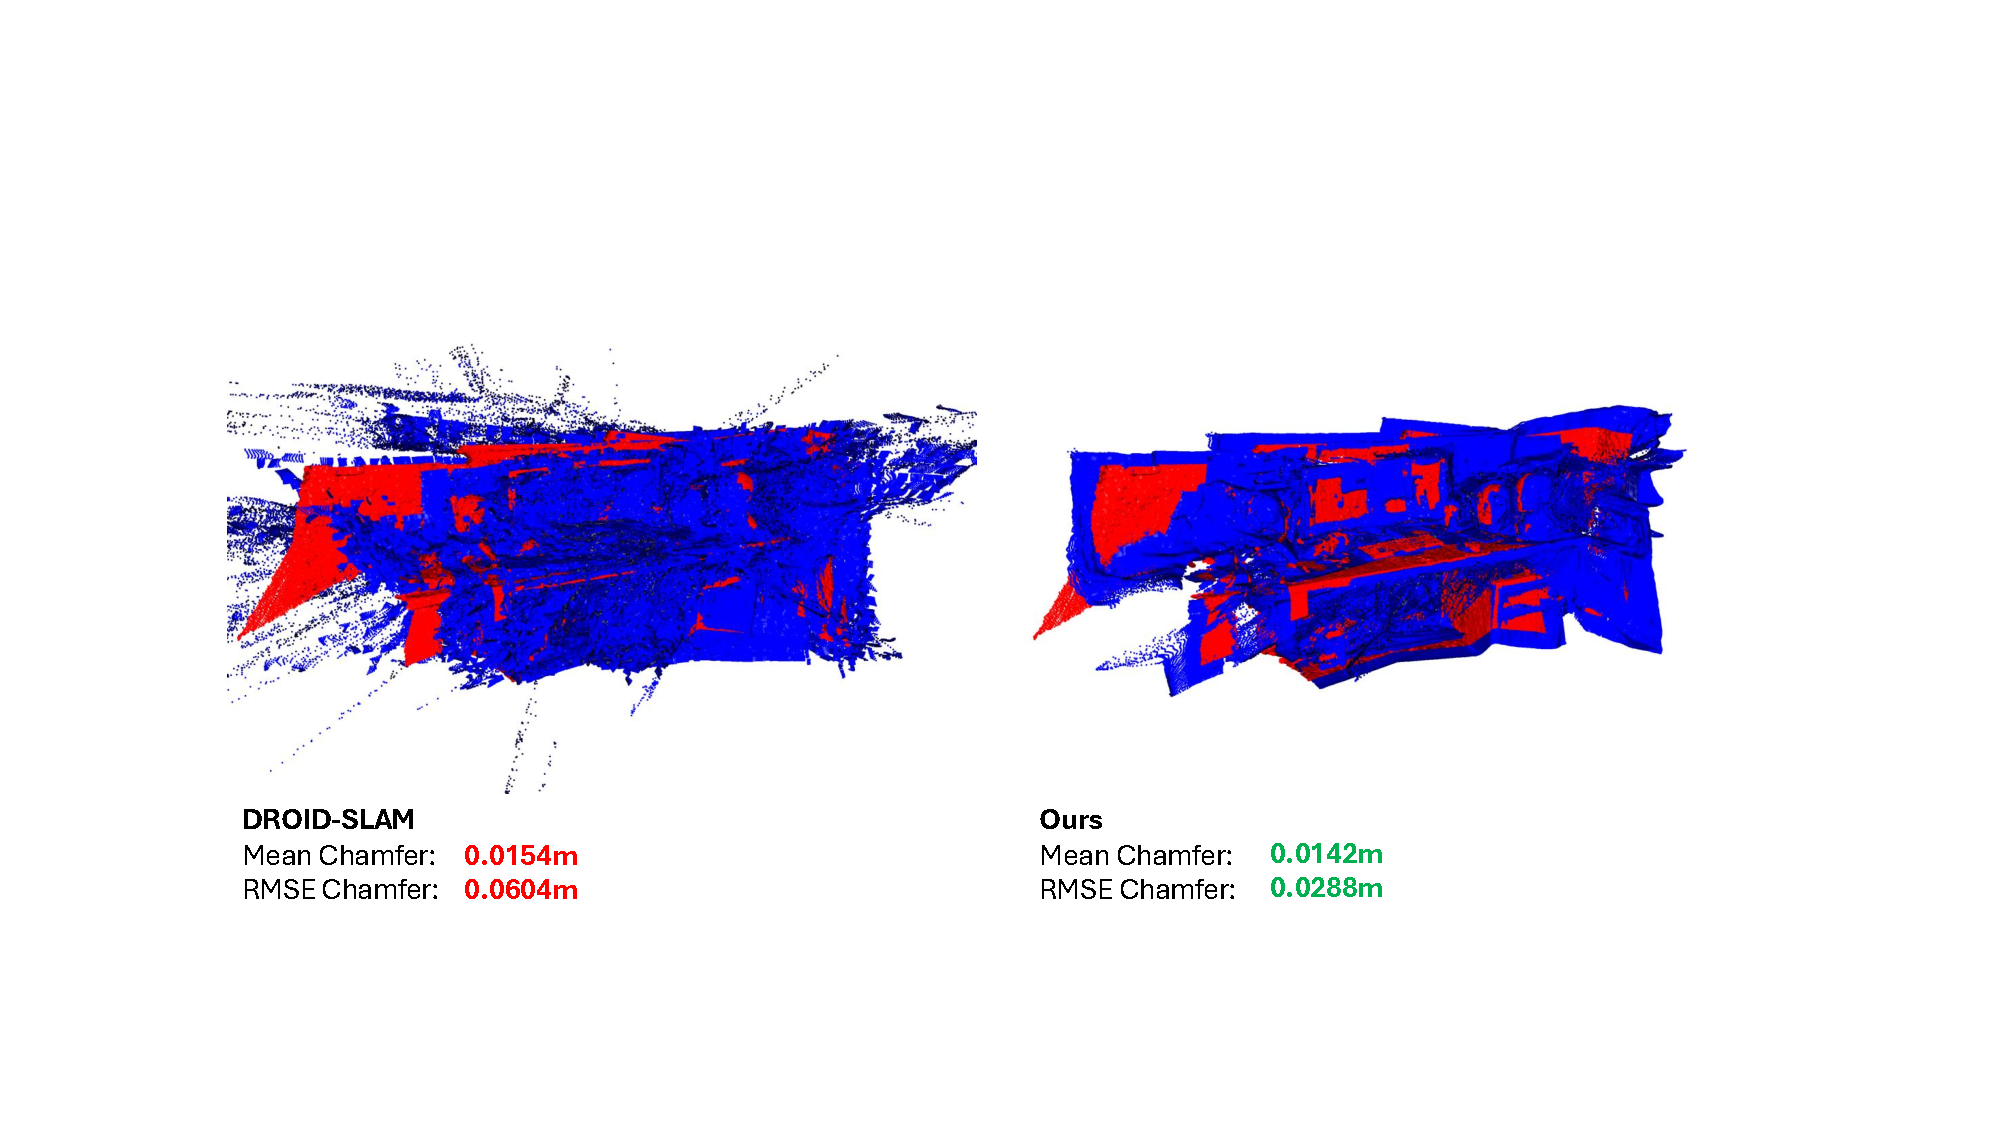
\includegraphics[width=\textwidth]{figs/7scenes_geometry.pdf}
    \caption{Reconstruction comparison on 7-Scenes heads, with red indicating the ground-truth point cloud and blue the estimated point cloud.  While mean Chamfer distance does not significantly penalise inconsistent points, RMSE Chamfer is a better reflection of the quality of the geometry.}
    \label{fig:7scenes_geometry}
\end{figure*}

\begin{figure*}[t]
    \centering
    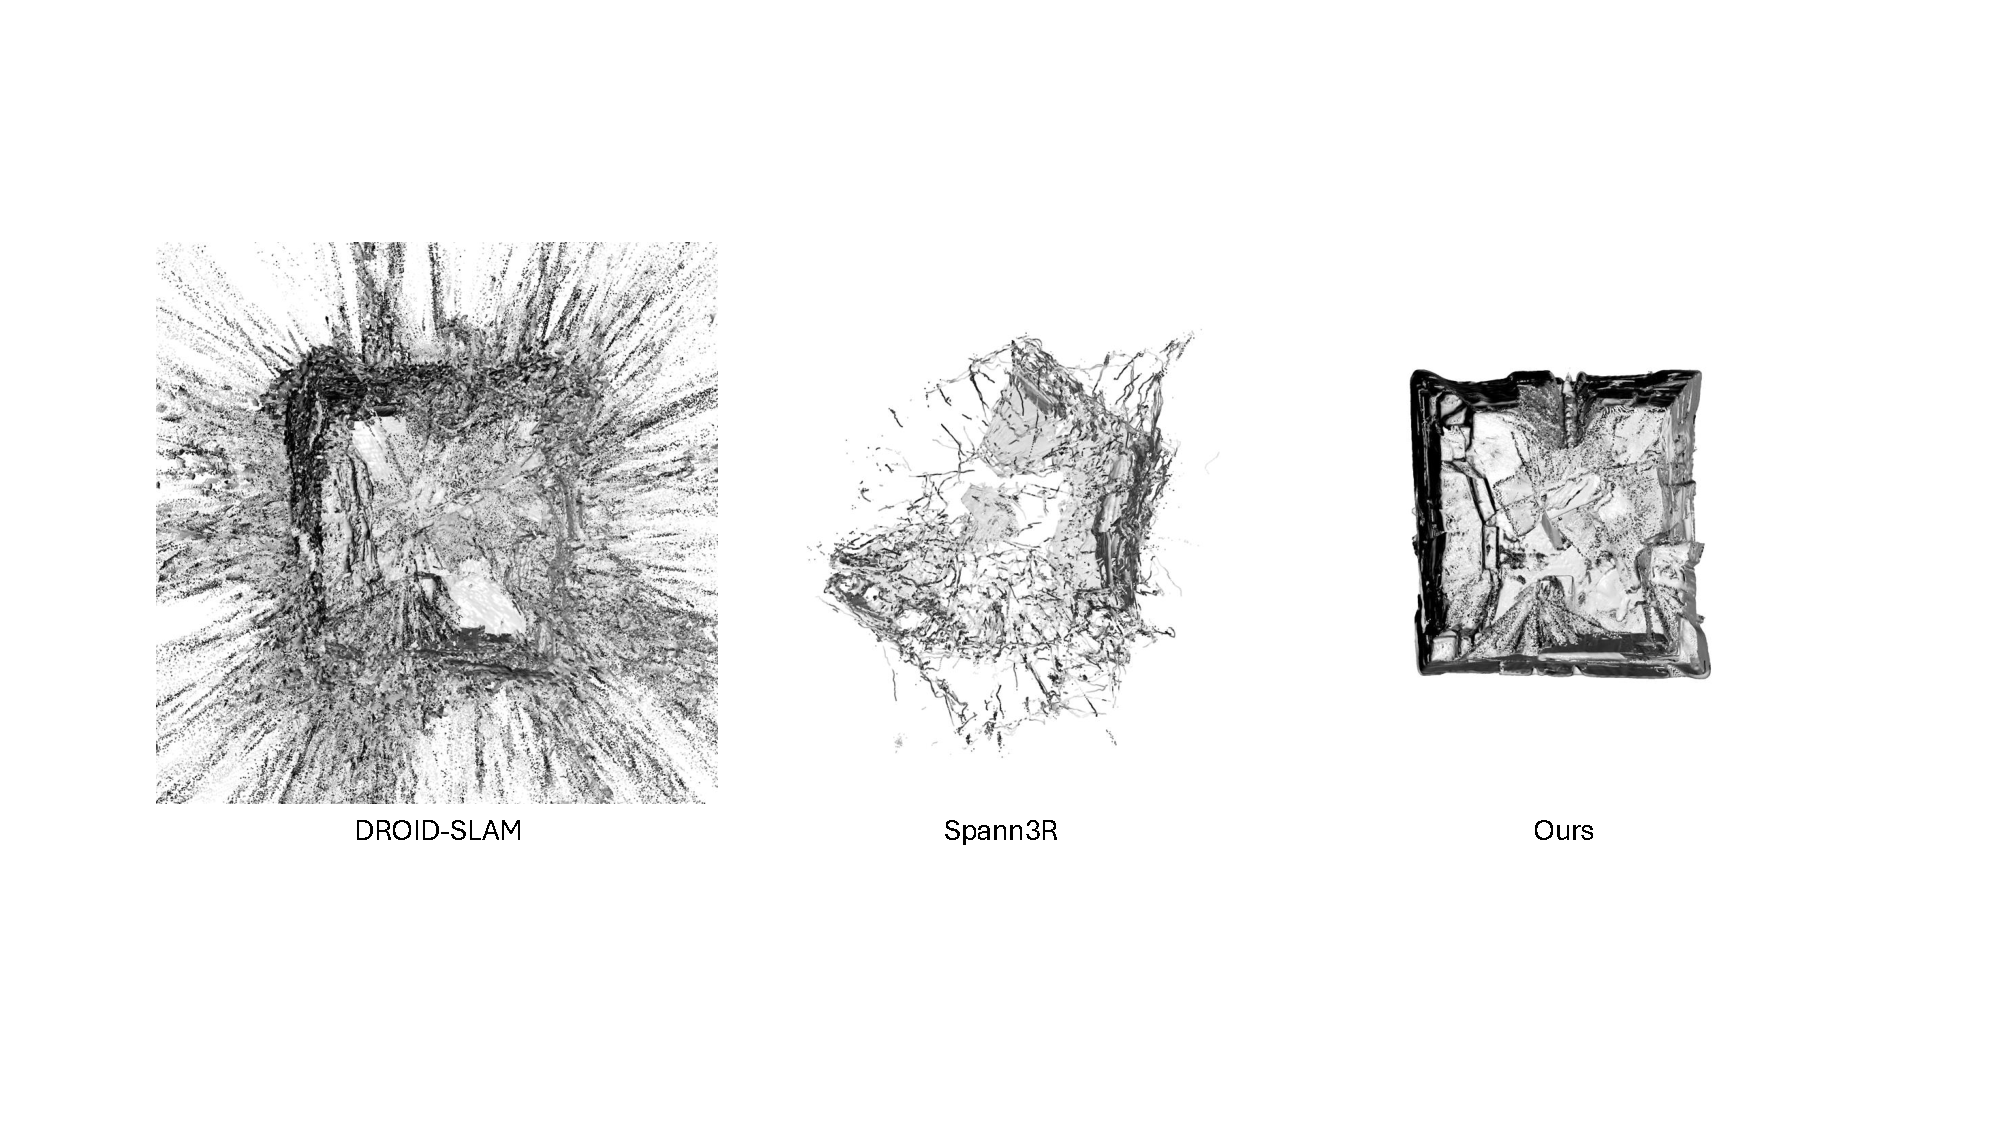
\includegraphics[width=\textwidth]{figs/euroc_geometry.pdf}
    \caption{Reconstruction comparison on EuRoC V102.}
    \label{fig:euroc_geometry}
\end{figure*}

\subsection{Trajectory Evaluation [\cref{sec:camera-pose-estimation}]]}
For all the datasets, we use the same parameters with keyframe threshold $\KFthreshold = 0.333$, loop-closure threshold $\LCthreshold= 0.1$, and $\Retrievalthreshold=0.005$.
For relocalisation, we have a stricter check to allow for the current frame to be attached to the graph.  The match fraction must be greater than 0.3 for all datasets apart from in ETH3D where we set the threshold higher to 0.5.

For trajectory evaluation, we run DROID-SLAM using the open-source code with the configuration files given for each dataset.  For 7-Scenes, we use the TUM configuration file since it is the most similar.  For TUM and EuRoC, the remaining entries are from the tables in Deep Patch Visual SLAM \cite{lipson2024deep}, which also uses some results from DROID-SLAM \cite{teed_droid_2021}.  For 7-Scenes, we include the results reported from NICER-SLAM \cite{zhu_nicer_2024}.  For ETH3D, we ran all methods locally as the dataset was not previously attempted with monocular SLAM methods.

\subsection{Geometry Evaluation [\cref{sec:dense-geometry-eval}]}
For evaluation, points that are unobservable are removed from the reference point cloud.
Additionally, for the 7-Scenes dataset, we filter out depths which are marked as invalid.
For all methods, we do not filter any estimated point, as in an incremental problem setting like SLAM, reprojection-based filtering is not always possible and downstream applications benefit from per-pixel dense prediction.


For the metrics, we report the RMSE which penalises outlying measurements.
\cref{fig:7scenes_geometry} is an illustrative example, where DROID-SLAM and \master-SLAM achieve a similar mean Chamfer distance.  Qualitatively, however, \master-SLAM clearly produces more coherent and accurate geometry, and this difference is reflected in the RMSE Chamfer distance.

\begin{table*}[t]\centering
\caption{Absolute trajectory error (ATE (m)) on EuRoC \cite{burri_euroc_2016}.}\label{tab:euroc_ate}
\footnotesize
\begin{tabular}{l|lcccccccccccc} %\toprule
& &MH01 &MH02 &MH03 &MH04 &MH05 &V101 &V102 &V103 &V201 &V202 &V203 &avg \\
\hline
\multirow{8}{*}{Calibrated} &\textbf{ORB-SLAM} &0.071 &0.067 &0.071 &0.082 &0.060 &\textbf{0.015} &0.020 &X &0.021 &0.018 &X &- \\
&\textbf{DeepV2D \cite{teed_deepv2d_2020}} &0.739 &1.144 &0.752 &1.492 &1.567 &0.981 &0.801 &1.570 &0.290 &2.202 &2.743 &1.298 \\
&\textbf{DeepFactors \cite{czarnowski_deepfactors_2020}} &1.587 &1.479 &3.139 &5.331 &4.002 &1.520 &0.679 &0.900 &0.876 &1.905 &1.021 &2.040 \\
&\textbf{DPV-SLAM \cite{lipson2024deep}} &\textbf{0.013} &0.016 &\underline{0.022} &\underline{0.043} &\textbf{0.041} &\underline{0.035} &\textbf{0.008} &\textbf{0.015} &0.020 &\underline{0.011} &0.040 &0.024 \\
&\textbf{DPV-SLAM++ \cite{lipson2024deep}} &\textbf{0.013} &0.016 &\textbf{0.021} &\textbf{0.041} &\textbf{0.041} &\underline{0.035} &\underline{0.010} &\textbf{0.015} &0.021 &\underline{0.011} &0.023 &\underline{0.023} \\
&\textbf{GO-SLAM \cite{zhang2023goslam}} &\underline{0.016} &\underline{0.014} &0.023 &0.045 &0.045 &0.037 &0.011 &0.023 &\textbf{0.016} &\textbf{0.010} &\underline{0.022} &0.024 \\
&\textbf{DROID-SLAM \cite{teed_droid_2021}} &\textbf{0.013} &\textbf{0.012} &\underline{0.022} &0.048 &\underline{0.044} &0.037 &0.013 &\underline{0.019} &\underline{0.017} &\textbf{0.010} &\textbf{0.013} &\textbf{0.022} \\
&\textbf{Ours} &0.023 &0.017 &0.057 &0.113 &0.067 &0.040 &0.019 &0.027 &0.020 &0.025 &0.043 &0.041 \\
\hline
Uncalibrated &\textbf{Ours*} &0.180 &0.124 &0.156 &0.282 &0.327 &0.101 &0.134 &0.096 &0.133 &0.100 &0.170 &0.164 \\
\bottomrule
\end{tabular}
\end{table*}

We report the qualitative result of EuRoC reconstruction in \cref{fig:euroc_geometry}. \spanner fails as the sequence is not object-centric, and DROID-SLAM produces many more outliers compared to \master-SLAM .  Compared to \spanner which maintains a memory buffer, our keyframing system ensures that viewed parts of the scene are not discarded.  Furthermore, our efficient global optimisation can create globally consistent maps in real-time.

\section{EuRoC Results}

We summarise the average ATE for EuRoC in the main paper, and show the results for each sequence in \cref{tab:euroc_ate}.  While our system does not outperform DROID-SLAM and methods that leverage its matching architecture, EuRoC has traditionally been challenging for monocular systems due to aggressive motion, large-scale trajectories, and varying exposure.  As noted previously, DROID-SLAM was trained with explicit greyscale augmentation which may account for the gap in performance.  Compared to previous systems with geometric priors, such as DeepV2D and DeepFactors, we demonstrate significant improvements in trajectory estimation.  Furthermore, the results from the main paper highlight the additional benefits of using such a prior, as the dense geometry is more accurate and consistent as shown in \cref{tab:geometry}, even for our uncalibrated system.

\section{Comparison to Other SLAM/SfM Methods}

\subsection{DROID and DPV SLAM}

Our system uses a two-view geometric prior in a modular system, while DROID and DPV SLAM learn a matching prior as part of an end-to-end system with differentiable bundle adjustment.  While these systems are very accurate for pose estimation, there are fundamental limitations for geometry and generality.

First, bundle adjustment cannot guarantee coherent geometry even with accurate poses, as it lacks smoothness regularisation and constraints under low parallax.  Given MASt3R, we find local fusion and scale optimisation to be sufficient for consistency and coherence, while the BA of DROID loses the latter.
Second, beyond improved geometry, geometric priors enable new capabilities like continuously changing intrinsics.  DROID fixes the model to pinhole during training, and also cannot efficiently handle time-varying intrinsics as this slows down backend optimisation.

\subsection{MASt3R-SfM}

MASt3R-SfM uses sparse correspondences (subsampling 1/64 pixels) due to MASt3R's brute-force matching.  Our dense projective pointmap matching formulates search as local optimisation and achieves a 1000x speedup without compromising accuracy as shown in \cref{tab:matching}. Global optimisation in MASt3R-SfM uses a 1st-order optimiser, lacks minimal rotation updates, and introduces degenerate solutions that require scale renormalisation.
To avoid such problems, we formulate a nonlinear least-squares problem and develop a 2nd-order optimiser with minimal pose updates and gauge fixing.
Our uncalibrated ray formulation achieves a similar accuracy as MASt3R-SfM's procedure of fitting pinhole models and minimising reprojection error, but we avoid selecting a specific camera model. This maintains generality of our SLAM system in order to handle all types of distortion, such as fisheye in the future.

% \section{Rationale}
% \label{sec:rationale}
% %
% Having the supplementary compiled together with the main paper means that:
% %
% \begin{itemize}
% \item The supplementary can back-reference sections of the main paper, for example, we can refer to \cref{sec:intro};
% \item The main paper can forward reference sub-sections within the supplementary explicitly (e.g. referring to a particular experiment);
% \item When submitted to arXiv, the supplementary will already included at the end of the paper.
% \end{itemize}
% %
% To split the supplementary pages from the main paper, you can use \href{https://support.apple.com/en-ca/guide/preview/prvw11793/mac#:~:text=Delete%20a%20page%20from%20a,or%20choose%20Edit%20%3E%20Delete).}{Preview (on macOS)}, \href{https://www.adobe.com/acrobat/how-to/delete-pages-from-pdf.html#:~:text=Choose%20%E2%80%9CTools%E2%80%9D%20%3E%20%E2%80%9COrganize,or%20pages%20from%20the%20file.}{Adobe Acrobat} (on all OSs), as well as \href{https://superuser.com/questions/517986/is-it-possible-to-delete-some-pages-of-a-pdf-document}{command line tools}.
